\chapter{Security Design}
\label{chap:security-design}

\section{Introduction}
Security is a primary quality attribute of modern multi-tenant Software-as-a-Service (SaaS) environments. For collaboration platforms like Nexus PM, maintaining data confidentiality, tenant isolation, and identity validation is critical to protecting user workspaces and sensitive project metadata.

The purpose of this chapter is to detail the security design of Nexus PM. It outlines the platform's security philosophy, access token lifecycles, role-based authorization matrices, data encryption standards, and threat mitigation models.

\section{Security Architecture}
The security architecture of Nexus PM is built on four core design philosophies:
\begin{itemize}
    \item \textbf{Defense in Depth:} Rather than relying on a single security boundary, the platform enforces validation checks at multiple layers, including transport encryption (TLS), gateway rate limiting, stateless JWT validation, service-layer role checks, and database-level relational integrity.
    \item \textbf{Least Privilege:} Users and service components are granted only the permissions required to execute their specific functions. Project roles restrict actions to those matching the user's role (e.g., Viewers cannot edit tasks).
    \item \textbf{Secure by Default:} Security controls are active by default. Authentication is required for all API endpoints unless explicitly flagged as public (e.g., login, register). Cookies default to maximum security settings.
    \item \textbf{Separation of Responsibilities:} Logical boundaries isolate core systems. File assets bypass the API compute threads, running directly to Cloudflare R2, and external integrations (e.g., Gemini AI, Resend) are managed separately from core database transactions.
\end{itemize}

\section{Authentication}
Authentication verifies user identities, supporting both local credentials and federated Google OAuth logins.

\subsection{Stateless JSON Web Tokens}
Upon successful authentication, the platform issues an asymmetric access token and a refresh token:
\begin{itemize}
    \item \textbf{Access Token:} A short-lived JWT (valid for 15 minutes) signed with HMAC-SHA256. It contains the user identity (\texttt{sub}), scope details, and a unique JWT ID (\texttt{jti}) to prevent replay attacks. Access tokens are validated statelessly by the API gateway.
    \item \textbf{Refresh Token:} A long-lived JWT (valid for 7 days) signed with a separate key. Unlike access tokens, refresh tokens must be verified against a database table to support manual session revocation and automated token rotation.
\end{itemize}

\subsection{Refresh Token Hashing}
To prevent database compromise from exposing active user sessions, refresh tokens are hashed using SHA-256 (\texttt{hash\_token}) before being stored in the database. When a client requests a new access token, the incoming refresh token is hashed and compared against the database records, protecting active sessions in the event of database dumps.

\subsection{OTP Verification Security}
For local user registration and password recovery workflows, the system enforces secure one-time password (OTP) verification:
\begin{itemize}
    \item \textbf{Cryptographic Hashing:} OTP codes are generated as random 6-digit integers, which are then hashed using SHA-256 before database insertion in the \texttt{password\_reset\_otps} table, protecting OTP credentials in the event of a database compromise.
    \item \textbf{Strict Expiration Limits:} OTP codes expire 15 minutes after generation. An automated background job running in the FastAPI lifecycle (\texttt{cleanup\_expired\_otps\_job}) runs every 24 hours to delete expired OTP records.
    \item \textbf{Rate-Limit Protections:} Brute-force guessing attacks on OTP validation are blocked by logging and checking request rates on the `/verify-otp` and `/forgot-password` routes using the database-backed \texttt{forgot\_password\_rate\_limits} log table.
\end{itemize}

\subsection{Cookie Security Specifications}
Tokens are returned to the client using secure cookies configured with strict attributes:
\begin{itemize}
    \item \texttt{HttpOnly} prevents client-side JavaScript from accessing cookies, mitigating Cross-Site Scripting (XSS) risks.
    \item \texttt{Secure} restricts cookie transmission to HTTPS channels, preventing token exposure over unencrypted networks.
    \item \texttt{SameSite} settings default to \texttt{Lax} (or configured via environment variables) to secure cookies on cross-origin requests, mitigating Cross-Site Request Forgery (CSRF) vulnerabilities.
\end{itemize}

\begin{figure}[h!]
    \centering
    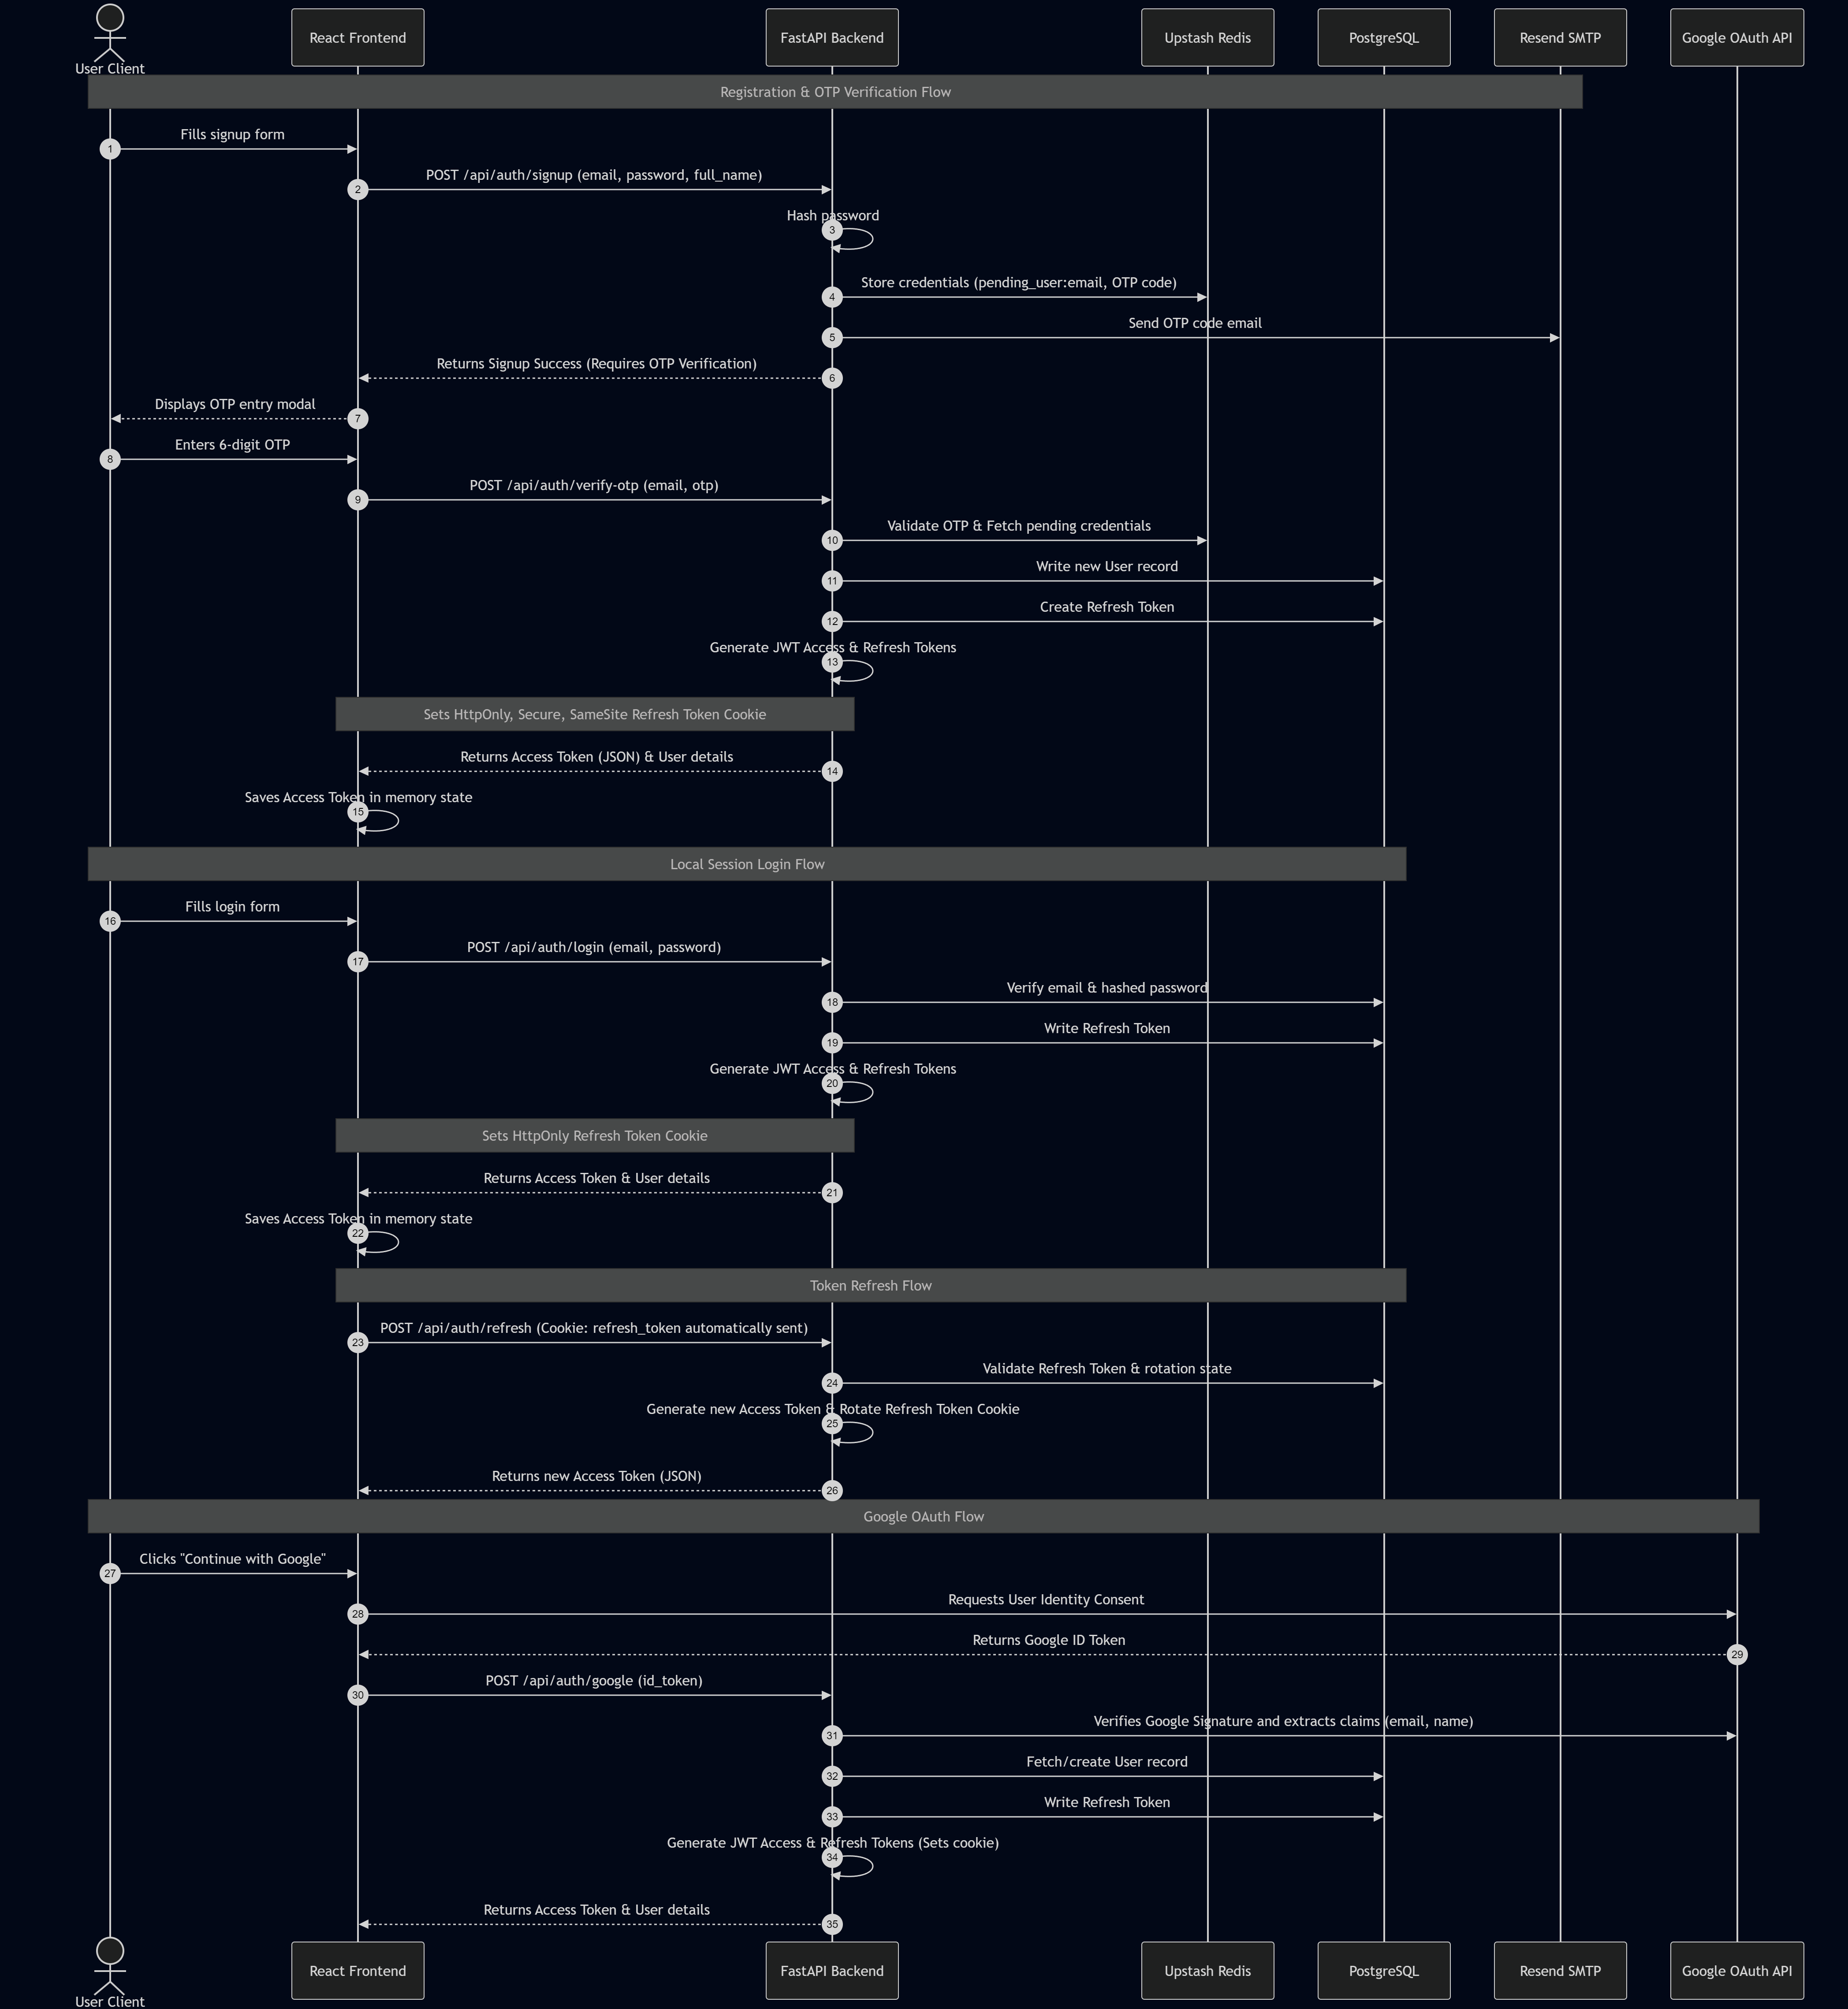
\includegraphics[width=\textwidth]{figures/authentication-flow.png}
    \caption{Nexus PM User Authentication and Token Verification Flow}
    \label{fig:auth_flow_diagram}
\end{figure}

\section{Authorization}
Authorization enforces data access boundaries and role-based permissions across workspaces and projects.

\subsection{Role-Based Access Control (RBAC)}
Access control is managed using project-level roles. A user's permissions within a project are determined by their role mapping in the \texttt{project\_members} table, as outlined in the authorization matrix in Table~\ref{tab:rbac_matrix}.

\begin{table}[h!]
\centering
\small
\renewcommand{\arraystretch}{1.4}
\begin{tabularx}{\textwidth}{l C C C C C C}
    \toprule[1.5pt]
    \rowcolor{primary!5}
    \textbf{\color{primary}Project Role} & \textbf{\color{primary}View Tasks} & \textbf{\color{primary}Create Tasks} & \textbf{\color{primary}Edit Tasks} & \textbf{\color{primary}Delete Tasks} & \textbf{\color{primary}Manage Members} & \textbf{\color{primary}Delete Project} \\
    \midrule
    \textbf{Owner}     & Yes & Yes & Yes & Yes & Yes & Yes \\
    \textbf{Manager}   & Yes & Yes & Yes & Yes & Yes & No  \\
    \textbf{Developer} & Yes & Yes & Yes & No  & No  & No  \\
    \textbf{Viewer}    & Yes & No  & No  & No  & No  & No  \\
    \bottomrule[1.5pt]
\end{tabularx}
\caption{Role-Based Access Control (RBAC) Permission Matrix}
\label{tab:rbac_matrix}
\end{table}

\subsection{Access Control Verification}
Permissions are validated dynamically before executing router handlers:
\begin{enumerate}
    \item The gateway parses the request to identify the target project ID.
    \item The service layer queries the \texttt{project\_members} table to verify that the user is an active member.
    \item The dependency injection handler evaluates the user's role against the endpoint's permitted roles.
    \item If validation fails, an HTTP 403 Forbidden exception is raised, terminating the request.
\end{enumerate}

\section{API Security}
Gateway security controls validate incoming requests and sanitize outgoing responses:
\begin{itemize}
    \item \textbf{Input Validation:} Request bodies are parsed against Pydantic schemas, enforcing type constraints and length limits before data reaches service logic.
    \item \textbf{Output Serialization:} Response models filter sensitive database columns (e.g., password hashes, Google IDs), preventing accidental data leaks.
    \item \textbf{Error Sanitation:} Global exception handlers capture raw database and service errors, returning generic error codes to clients while writing detailed diagnostic traces to secure server logs.
\end{itemize}

\section{Data Security}
Data security controls protect information at rest and in transit:
\begin{itemize}
    \item \textbf{Credential Hashing:} Local user passwords are encrypted using the bcrypt key-derivation function. The system uses a work factor of 12 rounds to resist brute-force attacks.
    \item \textbf{Secrets Management:} Private API keys, database URLs, and JWT keys are stored as system environment variables and loaded at runtime, preventing hardcoded credentials in code repositories.
    \item \textbf{Transport Layer Encryption:} All network traffic is encrypted using TLS 1.3, protecting session cookies and API tokens from interception.
\end{itemize}

\section{File Storage Security}
The storage module manages file attachments by coordinating direct uploads to Cloudflare R2, keeping large file streams off the API backend:
\begin{itemize}
    \item \textbf{Pre-Signed URL Constraints:} Upload authorization is restricted by generating pre-signed URLs with a 15-minute expiration window.
    \item \textbf{Size and Type Validation:} Before generating upload URLs, the backend validates that file sizes are under limits (e.g., 10MB) and MIME types match a whitelist (e.g., PDF, PNG, JPEG), blocking execution of malicious scripts.
    \item \textbf{Direct Upload Bypass:} Direct uploads to R2 prevent backend thread blocks, reducing vulnerability to denial-of-service (DoS) resource exhaustion attacks.
\end{itemize}

\section{External Service Security}
Integrating external managed services requires secure communication boundaries:
\begin{itemize}
    \item \textbf{Supabase (PostgreSQL):} Connections use secure SSL/TLS, and connection pooling (PgBouncer) transaction modes are utilized to prevent connection exhaustion.
    \item \textbf{Cloudflare R2:} Requests use AWS Signature Version 4 protocols, validating authorization keys on every API interaction.
    \item \textbf{Upstash Redis:} Access requires password authentication over TLS, securing rate-limiting and session cache operations.
    \item \textbf{Resend \& Gemini AI:} Communication with email and LLM gateways runs over secure HTTPS API endpoints using validated API keys.
\end{itemize}

\pagebreak
\section{Threat Analysis}
The Nexus PM design implements mitigations to address common security threats, as detailed in Table~\ref{tab:threat_mitigation}.

\begin{table}[h!]
\centering
\small
\renewcommand{\arraystretch}{1.4}
\begin{tabularx}{\textwidth}{l X X}
    \toprule[1.5pt]
    \rowcolor{primary!5}
    \textbf{\color{primary}Threat Name} & \textbf{\color{primary}System Impact} & \textbf{\color{primary}Nexus PM Mitigation} \\
    \midrule
    Unauthorized API Access & Leakage of workspace data & Stateless JWT verification enforced across all endpoints. \\
    Privilege Escalation & Unauthorized task modifications & Route permissions checked using dependency injection. \\
    Token Theft (XSS/CSRF) & Account takeover via hijacked tokens & Access tokens isolated, and refresh tokens secured in HttpOnly cookies. \\
    SQL Injection & Database data exposure or theft & SQL parameterization enforced using the SQLAlchemy ORM. \\
    File Upload Abuse & Script execution in browser contexts & Size validation and MIME-type checks verified before upload. \\
    Rate Abuse & Denial-of-Service (DoS) events & API rate limits tracked in Upstash Redis. \\
    Credential Compromise & Session takeover via database dump & Password hashing using bcrypt and refresh token hashing using SHA-256. \\
    \bottomrule[1.5pt]
\end{tabularx}
\caption{Threat Analysis and Architectural Mitigations Matrix}
\label{tab:threat_mitigation}
\end{table}

\section{Security Best Practices}
The platform incorporates secure software engineering practices:
\begin{itemize}
    \item \textbf{Dependency Vulnerability Checks:} Container builds use multi-stage Docker configurations to reduce the attack surface, and dependency vulnerability scans (e.g., Snyk or Dependabot) are run regularly.
    \item \textbf{X-Request-ID Tracking:} Every API interaction is logged with a trace identifier, supporting security auditing and diagnostics without logging sensitive user data.
\end{itemize}

\section{Future Security Enhancements}
Future iterations of the platform plan to incorporate several security enhancements:
\begin{itemize}
    \item \textbf{Multi-Factor Authentication (MFA):} Implement Time-based One-Time Passwords (TOTP) to secure local password logins.
    \item \textbf{HTTP Security Headers:} Configure Content Security Policies (CSP), HTTP Strict Transport Security (HSTS), and framing protections (\texttt{X-Frame-Options}) at the frontend hosting layer.
    \item \textbf{Automated Secrets Rotation:} Implement automated secret keys and database credential rotation workflows using cloud vault managers.
\end{itemize}

\section{Chapter Summary}
This chapter detailed the security design of the Nexus PM platform, specifying its authentication standards, role-based authorization matrices, API validations, and external integration protections. By using secure cookies, hashing credentials, and validating file uploads, the architecture protects sensitive project metadata and ensures tenant isolation. The next chapter will focus on the testing strategies used to verify these security controls and system functionality.
